\chapter[Análisis de Requisitos]{Análisis de Requisitos globales}

En este capítulos explicaremos el proceso de análisis de requisitos llevados a cabo para la elaboración de la aplicación y toda la información recibida por la comunidad.

\section{Consultas con la comunidad}

\paragraph{Blabla} Blabla

\subsection{Resumen}
	\paragraph{Blabla} Blabla

\section{Análisis de otros elementos}
Otros proyectos de accesbilidad o juegos.

\section{Requisitos del aplicativo}
Con toda la información obtenida y pensada, creamos una lista con los casos de uso que nuestro proyecto debe de cumplir.

\begin{itemize}
  \item \textbf{Whatever} Blabla
\end{itemize}

FIGURA DE CASOS DE USO UML. Hacer referencia.

% \begin{figure}[h!]
%     \centering
%     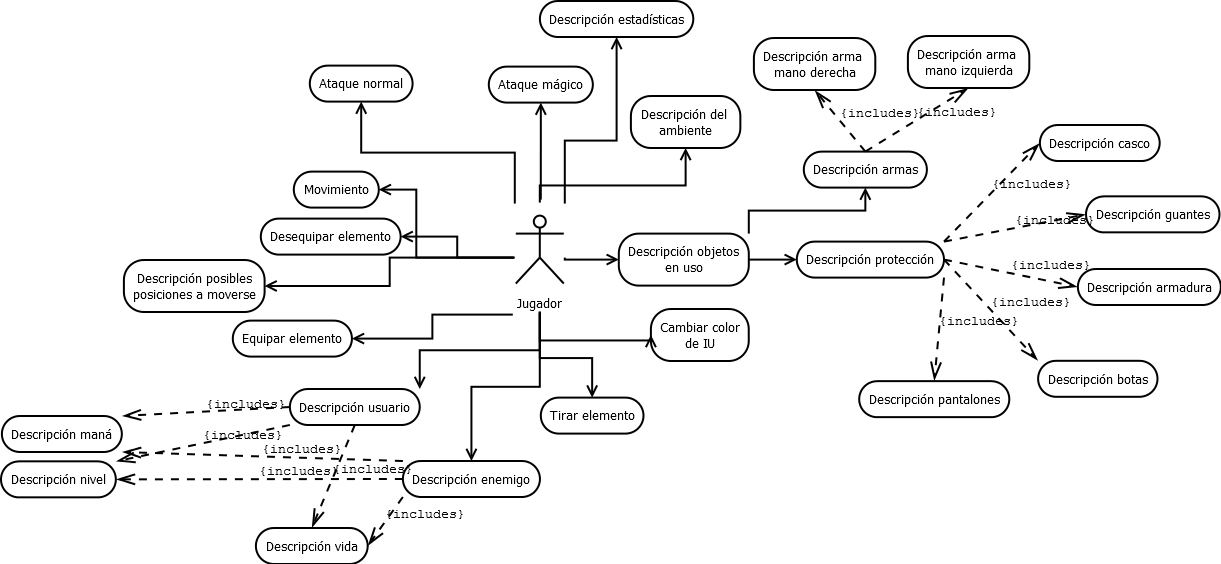
\includegraphics[width=0.9\textheight,angle=90]{img/casosdeuso.png}
%     \caption{Diagrama UML de casos de uso de la aplicación}
%     \label{fig:casosdeuso}
% \end{figure}
